\documentclass[11pt,a4paper]{article}
\usepackage[T1]{fontenc}
\usepackage[utf8]{inputenc}
\usepackage{lmodern}
\usepackage[margin=2.4cm]{geometry}
\usepackage{microtype}
\usepackage{xcolor}
\usepackage{booktabs}
\usepackage{longtable}
\usepackage{array}
\newcolumntype{L}[1]{>{\raggedright\arraybackslash}p{#1}}
\usepackage{enumitem}
\usepackage{fancyhdr}
\usepackage{titlesec}
\usepackage{tikz}
\usetikzlibrary{arrows.meta,positioning,shapes.geometric,fit,backgrounds}
\usepackage[colorlinks=true,linkcolor=accent,urlcolor=accent,citecolor=accent]{hyperref}

\definecolor{accent}{HTML}{4F46E5}
\definecolor{soft}{HTML}{ECEAFD}
\definecolor{warn}{HTML}{A15C00}
\definecolor{good}{HTML}{157A4A}

\newcommand{\leotex}{Leo\TeX{}}
\newcommand{\key}[1]{\texttt{\small #1}}
\newcommand{\fpath}[1]{\texttt{\small #1}}
\newenvironment{note}{\par\medskip\noindent\begin{tabular}{|p{0.955\linewidth}}\color{accent}\textbf{Note.} }{\end{tabular}\par\medskip}
\newenvironment{caution}{\par\medskip\noindent\begin{tabular}{|p{0.955\linewidth}}\color{warn}\textbf{Careful.} }{\end{tabular}\par\medskip}

\titleformat{\section}{\Large\bfseries\color{accent}}{\thesection}{0.6em}{}
\titleformat{\subsection}{\large\bfseries}{\thesubsection}{0.6em}{}
\setlist{itemsep=2pt,topsep=4pt}
\setlength{\parskip}{4pt}
\setlength{\parindent}{0pt}
\pagestyle{fancy}
\fancyhf{}
\fancyhead[L]{\leotex{} guide}
\fancyhead[R]{\thepage}
\renewcommand{\headrulewidth}{0.3pt}
\setlength{\headheight}{14pt}
\emergencystretch=3em

\begin{document}

\begin{titlepage}
\centering
\vspace*{3cm}
{\fontsize{56}{60}\selectfont\bfseries\color{accent}\leotex{}}\par
\vspace{0.6cm}
{\Large A free online \LaTeX{} editor with a complete \TeX{} Live behind it}\par
\vspace{1.2cm}
{\large The complete guide: how it works, how to use it, how to set it up,\\ how it is kept safe and how to keep it running}\par
\vfill
\begin{tabular}{rl}
Version & 1.3.0 (22 November 2026)\\
Live site & \url{https://prism-latex.github.io/prism-app/}\\
Source & \url{https://github.com/prism-latex/prism-app}\\
Licence & MIT
\end{tabular}
\vspace{2cm}
\end{titlepage}

\tableofcontents
\clearpage

%% ------------------------------------------------------------------
\section{What \leotex{} is}

\leotex{} (written like \TeX{}, with the lowered E) is a website for writing \LaTeX{} documents. You type in the browser, press
\emph{Compile}, and read the finished PDF next to your text. It replaces a hosted \LaTeX{} editor that was shut down, and it is built
so that nobody can shut it down again: there is no company server in the middle.

\begin{itemize}
  \item \textbf{The page} is a static website on GitHub Pages. It is just program code; it holds no documents.
  \item \textbf{Your projects} live in a \emph{private GitHub repository that you own}, with the full history of every change.
  \item \textbf{Compiling} happens in GitHub Actions, on a machine with a complete \TeX{} Live. There is no page limit, no package limit
        and no ``compile timeout'' beyond the one you set yourself.
  \item \textbf{Accounts} are optional. They let you sign in on a new browser with email and password, Google or GitHub, instead of
        typing your GitHub token again.
\end{itemize}

\begin{figure}[h]
\centering
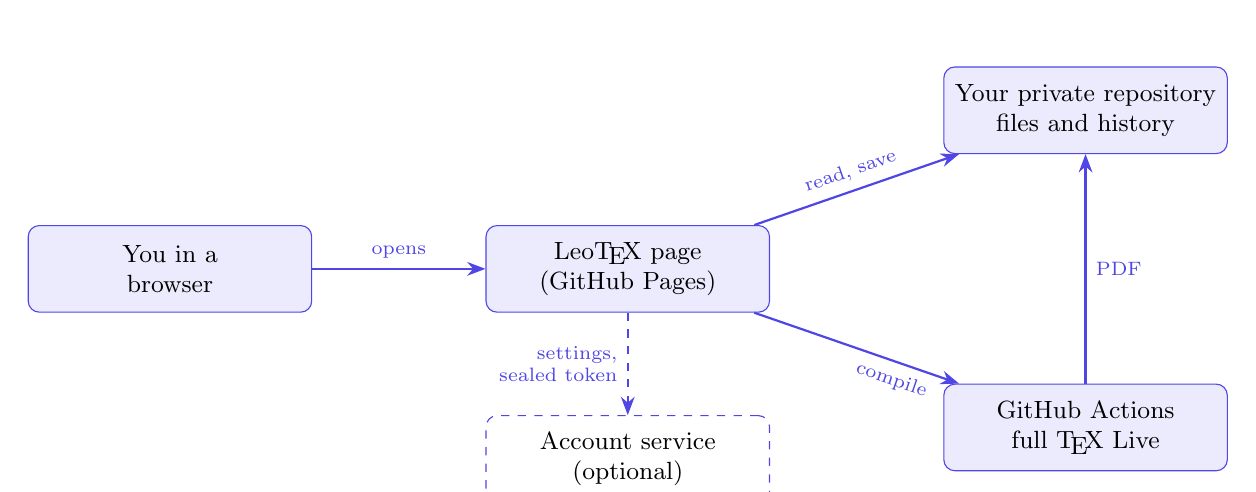
\begin{tikzpicture}[
  box/.style={draw=accent,fill=soft,rounded corners=4pt,align=center,minimum width=3.6cm,minimum height=1.1cm,font=\small},
  opt/.style={draw=accent,dashed,fill=white,rounded corners=4pt,align=center,minimum width=3.6cm,minimum height=1.1cm,font=\small},
  arr/.style={-{Stealth},thick,accent}]
\node[box] (you) {You in a\\browser};
\node[box,right=2.2cm of you] (page) {\leotex{} page\\(GitHub Pages)};
\node[box,above right=0.9cm and 2.2cm of page] (gh) {Your private repository\\files and history};
\node[box,below right=0.9cm and 2.2cm of page] (act) {GitHub Actions\\full \TeX{} Live};
\node[opt,below=1.3cm of page] (acc) {Account service\\(optional)};
\draw[arr] (you) -- node[above,font=\scriptsize]{opens} (page);
\draw[arr] (page) -- node[above,sloped,font=\scriptsize]{read, save} (gh);
\draw[arr] (page) -- node[below,sloped,pos=0.7,font=\scriptsize]{compile} (act);
\draw[arr] (act) -- node[right,font=\scriptsize]{PDF} (gh);
\draw[arr,dashed] (page) -- node[left,font=\scriptsize,align=right]{settings,\\sealed token} (acc);
\end{tikzpicture}
\caption{The parts. Your documents only ever travel between the page and your own repository.}
\end{figure}

\section{Quick start}
\begin{enumerate}
  \item Open \url{https://prism-latex.github.io/prism-app/}.
  \item On GitHub, create a \textbf{private} repository (for example \fpath{prism-data}) and tick \emph{Add a README file}.
  \item Create a \textbf{fine-grained token} (GitHub $\rightarrow$ Settings $\rightarrow$ Developer settings $\rightarrow$ Fine-grained tokens).
        Repository access: only that repository. Permissions: \emph{Contents}, \emph{Actions} and, for the first set-up only, \emph{Workflows}, all
        \emph{Read and write}. Note the expiry date.
  \item In \leotex{}, press \emph{Connect repository}, enter owner, repository, branch (\fpath{main}) and the token. Choose how the token is
        kept (see section~\ref{sec:token}). Enter the expiry date to get a reminder ten days before it ends.
  \item Press \emph{Set up} in the yellow banner. This stores the compile workflow in your repository. Afterwards remove the
        \emph{Workflows} permission from the token.
  \item Press \emph{New project}, pick a template, write, press \emph{Compile}.
\end{enumerate}

\section{Using the editor}

\subsection{The start page}
After connecting you see all your projects as cards: name, engine (pdf\LaTeX{}, Xe\LaTeX{} or Lua\LaTeX{}), ``edited \ldots{} ago'' and a badge when
something is not saved yet. You can search, sort, and open a project with one click. Each card has a menu: \emph{rename}, \emph{duplicate},
\emph{download as ZIP}, \emph{delete}. Nothing reaches GitHub until you press \emph{Save}, and the history keeps old versions.

\emph{New project} offers nine templates: Article, Article with bibliography, Report/thesis, Beamer slides, Letter, Greek article, TikZ/PGFPlots
figures, code listings and Blank. \emph{Upload ZIP} imports an existing project: a wrapper folder is removed, junk is skipped, and the main file
and engine are detected. You can also drop a ZIP onto the page.

\subsection{Writing, with suggestions}
The editor highlights \LaTeX{} and helps while you type. Suggestions appear on their own; \key{Ctrl+Space} asks for them.
\textbf{Both \texttt{\textbackslash cite} and \texttt{/cite} work}: a slash after a space, followed by at least three letters, is treated like a
backslash, and picking the command replaces the slash.

\begin{longtable}{@{}L{4.6cm}L{10.2cm}@{}}
\toprule
\textbf{You type} & \textbf{What happens}\\\midrule\endhead
\texttt{\textbackslash cite} or \texttt{/cite}, Enter & inserts \verb|\cite{}| with the cursor inside and immediately lists the entries of your \fpath{.bib} files\\
inside \verb|\cite{| & every source with ``author year'', the title in a side panel; type any part of the key, an author, the year or a title word to narrow the list\\
\verb|\ref{|, \verb|\eqref{|, \verb|\cref{| & the labels defined anywhere in the project\\
\verb|\usepackage{| & about 150 common packages; \verb|\documentclass{|, \verb|\bibliographystyle{|, \verb|\usetikzlibrary{| have their own lists\\
\verb|\includegraphics{|, \verb|\input{|, \verb|\include{| & your images, respectively your \fpath{.tex} files\\
\verb|\bibliography{|, \verb|\addbibresource{| & your \fpath{.bib} files\\
\verb|\begin{|, Enter & the environment name, then the matching \verb|\end{...}| on its own line, cursor in between\\
\verb|\end{| & the environment that is still open first\\
any command, for example \texttt{/frac}, \texttt{/textbf} & the command with blanks for its arguments; Tab jumps from blank to blank\\
\verb|\alpha|, \verb|\leq|, \verb|\rightarrow| \ldots & more than 400 commands and symbols; Greek letters and operators show their glyph\\
\verb|\figure|, \verb|\table|, \verb|\equation|, \verb|\align|, \verb|\itemize|, \verb|\enumerate|, \verb|\frame|, \verb|\tikz|, \verb|\plot|, \verb|\code|, \verb|\theorem| & ready-made blocks\\
\bottomrule
\end{longtable}
Suggestions can be switched off under \emph{Settings $\rightarrow$ Editor}.

\subsection{Searching, outline, history}
The side panel has three tabs. \emph{Files}: the project tree with upload, new file, rename or move, delete, download, drag and drop.
\emph{Outline}: chapters and sections across all \verb|\input|/\verb|\include| files; a click jumps there. \emph{Search}: the whole project, plain or as
a regular expression, with \emph{Replace all} (stays local until you save). The clock button shows the history of the open file with a coloured
comparison and a one-click restore.

\subsection{The PDF}
The PDF has selectable text and clickable contents, references, citations and web addresses. Use the page box, zoom and download. \emph{Stop}
cancels a running compile. \textbf{SyncTeX works both ways:} double-click in the PDF (or Ctrl/Cmd-click, your choice in the settings) to jump to the
source line; \emph{Show this line in the PDF} scrolls to and highlights the spot. A switch makes the PDF follow your cursor.

\subsection{Saving, conflicts and compiling}
\emph{Save} is one commit in your repository. If someone else (another device, Codex, Claude) changed the branch meanwhile, edits to
\emph{different} files are merged automatically; for the \emph{same} file \leotex{} asks which version to keep and never overwrites
silently. Unsaved text survives a reload (it is kept in the browser). \emph{Compile} saves, starts the workflow, shows the PDF and a log with clickable
errors. Returning to the tab loads changes that were pushed from elsewhere.

\subsection{Compiler settings}
\emph{Compiler} on the start page sets, for the whole repository, the \textbf{\TeX{} Live version} (latest, or a frozen year from 2025 back to 2013, so a
document compiles exactly as it did then) and the \textbf{time limit} (1--40 minutes). They are saved as \fpath{prism-compiler.json}. Per project
(\emph{Project settings}): engine, main file, \emph{clean build}, extra latexmk options, use of the project's own \fpath{.latexmkrc} (needed for glossaries and custom
steps) and shell escape (for packages such as pythontex). Everything runs in an isolated container. After a compile the bar shows the \TeX{} Live year that
was used and the exact latexmk command.

\begin{note}Not available: programs that are not part of \TeX{} Live, such as Inkscape (package \texttt{svg}), Python libraries, Typst or Pandoc.\end{note}

\section{The settings page}
Open it from the round avatar at the top right (\emph{Settings}), or with \key{Ctrl+,}.
\begin{description}[leftmargin=3.2cm,style=nextline]
  \item[Profile] Display name and a picture. The image is cut to a square and shrunk to $160\times160$ pixels in your browser, so only a few kilobytes are stored.
  \item[Appearance] Light, dark or follow the system; seven accent colours (indigo, blue, teal, green, orange, rose, slate); editor font (monospace, serif,
        sans-serif) and size.
  \item[Editor] Suggestions on or off, line numbers, line wrapping, spell-check and its language, what click in the PDF jumps to the source, PDF follows the cursor.
  \item[Shortcuts] See below.
  \item[Connection] Which repository and branch you are using, how the token is kept, its expiry date, \emph{Change connection} and \emph{Clear this browser}.
  \item[Account] Sign in or out, save or remove the connection in your account, change the password, delete the account.
  \item[About] Version, licence, links.
\end{description}

\subsection{Keyboard shortcuts}
Press \emph{Change} next to an action, then press the new keys. Use Ctrl (Cmd on a Mac) or Alt with a key; a lone letter is refused. Keys that browsers or the
editor need (for example Ctrl+W, Ctrl+T, Ctrl+Z) are refused, and a combination already used for another action is reported instead of silently replaced.
\emph{Reset} restores one default, \emph{Reset all} restores all of them.

\begin{center}
\begin{tabular}{@{}lll@{}}
\toprule
\textbf{Action} & \textbf{Default} & \textbf{Works}\\\midrule
Save to GitHub & \key{Ctrl+S} & everywhere\\
Save and compile & \key{Ctrl+Enter} & everywhere\\
Show this line in the PDF & \key{Ctrl+Alt+J} & in the editor\\
Search in the whole project & \key{Ctrl+Shift+F} & in a project\\
Back to all projects & \key{Ctrl+Alt+H} & everywhere\\
Open settings & \key{Ctrl+,} & everywhere\\
Bold around the selection & \key{Ctrl+B} & in the editor\\
Emphasis around the selection & \key{Ctrl+I} & in the editor\\
Inline math around the selection & \key{Ctrl+Alt+M} & in the editor\\
\bottomrule
\end{tabular}
\end{center}
Not remappable and always available in the editor: \key{Ctrl+F} (find), \key{Ctrl+/} (comment), \key{Ctrl+Z}/\key{Ctrl+Y} (undo, redo).
Your changes are kept in the browser and, with an account, on every browser you sign in on.

\section{Accounts: sign in instead of typing the token again}
\label{sec:accounts}

\subsection{The problem and the idea}
Without an account a new browser knows nothing: you would enter repository and token again. \leotex{} therefore offers optional accounts. After you
sign up (once) and \emph{save your connection to your account}, any new browser needs only:
\begin{enumerate}
  \item \textbf{Sign in}: with email and password, with Google, or with GitHub.
  \item \textbf{Your vault passphrase}, once per browser, \emph{only if} you chose to protect the saved connection with one. With the ``sign-in only'' choice there is no second step.
\end{enumerate}
Then your repository opens, and your settings, shortcuts, name and picture are already in place.

\subsection{What the account service knows}
\begin{center}
\begin{tabular}{@{}L{5.3cm}L{9.6cm}@{}}
\toprule
\textbf{Data} & \textbf{Who can read it}\\\midrule
Email, hashed password or Google/GitHub identity & the account service (that is what an account is)\\
Display name, picture, preferences, shortcuts & the account service\\
Repository, branch and \textbf{token}, if you press \emph{Save my connection} & your choice. \emph{Sign-in only}: stored readable, so whoever reaches the account record or steals the session gets the token. \emph{With a passphrase}: nobody but you, encrypted in your browser first (AES-256-GCM, PBKDF2 with 600\,000 rounds)\\
Your \LaTeX{} files, PDFs, logs & never sent to the account service; only your repository holds them\\
\bottomrule
\end{tabular}
\end{center}
The vault passphrase is \emph{separate} from the account password on purpose. The service handles passwords when you type them, so a key made from the
password would not be secret from it. The passphrase never leaves your browser. \textbf{It cannot be recovered:} if you forget it, remove the saved connection
(\emph{Settings $\rightarrow$ Account}) and save it again with a new passphrase.

\subsection{Signing up and signing in}
\begin{itemize}
  \item \textbf{Create account} (email): enter email and a password of at least 8 characters. A confirmation email follows (turned on by default); open its
        link, then sign in. If you open the link on another device, the address is confirmed and you simply sign in there.
  \item \textbf{Google} or \textbf{GitHub}: one button, the provider asks you to agree, and you come back signed in. If the provider's verified email equals the
        address of an existing account, they become the same account, so you can sign up one way and sign in another.
  \item \textbf{Forgot your password?} sends a link; open it in the same browser and choose a new password.
  \item \textbf{Sign out} ends the session. It does \emph{not} remove the token from the browser; on a shared computer use \emph{Clear this browser}.
\end{itemize}

\subsection{The first time, step by step}
\begin{enumerate}
  \item Connect with your token as in the quick start.
  \item Menu (avatar) $\rightarrow$ \emph{Sign in or create an account}; sign up.
  \item \emph{Settings $\rightarrow$ Account $\rightarrow$ Save my connection to my account}; choose a passphrase (8+ characters), type it twice.
  \item On any other browser: open \leotex{}, sign in, type the passphrase, choose how this browser keeps the token (on the device, encrypted with
        the same passphrase, or only until the tab closes). Done.
\end{enumerate}

\subsection{Setting up the account service (owner, once)}
\label{sec:owner}
The page has no server, so the person who runs the site creates a free project at Supabase (\url{https://supabase.com}). It takes about fifteen minutes.
\begin{enumerate}
  \item Create the project (choose a region close to you). Keep the database password safe; \leotex{} does not use it.
  \item \emph{SQL Editor} $\rightarrow$ new query $\rightarrow$ paste the file \fpath{supabase/setup.sql} from the repository $\rightarrow$ \emph{Run}. It creates one table with
        row-level security (each user reaches only their own row), a ``delete my account'' function and a harmless \texttt{ping} function.
  \item \emph{Project Settings $\rightarrow$ API}: copy the \textbf{Project URL} and the \textbf{anon / publishable} key. Never use the \emph{service\_role} / secret key; the
        build refuses it.
  \item \emph{Authentication $\rightarrow$ URL Configuration}: Site URL \url{https://prism-latex.github.io/prism-app/}; add the same address under \emph{Redirect URLs}.
  \item \emph{Authentication $\rightarrow$ Providers}: switch \textbf{Email} on. For \textbf{GitHub}: GitHub $\rightarrow$ Settings $\rightarrow$ Developer settings $\rightarrow$ OAuth Apps $\rightarrow$
        \emph{New}; homepage as above, callback \url{https://<project-ref>.supabase.co/auth/v1/callback}; copy Client ID and secret into Supabase. For \textbf{Google}:
        Google Cloud Console $\rightarrow$ APIs \& Services $\rightarrow$ Credentials $\rightarrow$ \emph{OAuth client ID} (Web application) with the same callback address; copy Client ID
        and secret into Supabase.
  \item In the repository, create \fpath{cloud.config.json} next to \fpath{package.json}:\\
        \verb|{ "url": "https://<project-ref>.supabase.co",|\\
        \verb|  "anonKey": "<public key>" }|\\
        Commit and push. GitHub Pages rebuilds the site; Settings $\rightarrow$ Account now shows accounts as available.
\end{enumerate}
\begin{caution}The anon key is public by design; the row-level security rules in \fpath{setup.sql} are what protect the data. Run that file before you
announce the site. A weekly workflow (\fpath{keepalive.yml}) sends one harmless request so a free project is not paused for inactivity; GitHub switches scheduled
workflows off after 60 days without any repository activity, so run it by hand now and then. The built-in Supabase email sender is limited to a few
messages per hour; add your own SMTP server in Supabase if many people sign up.\end{caution}

\section{How the token is kept}
\label{sec:token}
\leotex{} needs a token to talk to your repository. A \emph{fine-grained} token limited to that one repository can read and change that repository's files and start compiles,
and nothing else. (If you enter a \emph{classic} token the app warns you, because it reaches all your repositories.) In this browser the token can be kept three ways:
\begin{description}[leftmargin=3.2cm,style=nextline]
  \item[On this device] Plain text in the browser's storage. Convenient: no questions. Readable by scripts running on the same site address, which is why \leotex{} lives alone in its
        own GitHub organisation.
  \item[Encrypted with a passphrase] Recommended. Asked once per restart. Unsaved drafts are encrypted too.
  \item[Only until the tab closes] Wiped when the tab closes. Most private.
\end{description}
\emph{Clear this browser} removes the token, drafts, preferences and the sign-in from this browser. If a device is lost, revoke the token on GitHub.

\section{Safety, privacy and rules}
\begin{itemize}
  \item \textbf{No third-party code.} The page's security policy allows scripts only from the site itself and connections only to \fpath{api.github.com} (plus the one account-service address if
        accounts are built in). No analytics, no advertising, no CDN. It refuses to run inside a frame (clickjacking).
  \item \textbf{Compiling is isolated.} Your \TeX{} code runs as untrusted: container without network, without privileges, non-root, with memory and time limits, and without any job credential.
        Only GitHub's own actions are used, pinned to exact versions.
  \item \textbf{Nothing is overwritten silently.} Saving is fast-forward only; conflicts are shown.
  \item \textbf{Inputs are treated as untrusted:} file names, log lines, PDF text and data coming back from the account service are inserted as text, never as markup; PDF links are limited to
        \texttt{http(s)} and \texttt{mailto}.
  \item \textbf{Rules of the platforms.} GitHub Actions is for building what is in the repository; compiling your own documents there is that use. Free private repositories include a monthly
        allowance of minutes (2\,000 at the time of writing). GitHub Pages sites are limited to 1\,GB and about 100\,GB of traffic a month and may not be used for commercial transactions. The
        current terms on GitHub's pages are what counts.
\end{itemize}

\section{Looking after it}
\begin{itemize}
  \item \textbf{Token expiry.} Enter the expiry date in the connection window; a banner appears ten days before. Create a new token, press \emph{Change connection}, paste it. If you saved the connection to
        your account, replace it afterwards (\emph{Settings $\rightarrow$ Account $\rightarrow$ Replace with the current connection}).
  \item \textbf{Working locally too.} Your repository is an ordinary Git repository: clone it, edit with any editor, push. The page sees pushes when you return to the tab or press \emph{Refresh}.
        Use \fpath{git pull} before editing and \fpath{git push} after.
  \item \textbf{Backups.} Every project's full history is in the repository; also keep a clone or a Git bundle on another disk.
  \item \textbf{Several people.} Each person uses their own repository (GitHub does not let a fine-grained token use someone else's personal repository). Share finished work by sending the PDF or ZIP, or
        by adding collaborators to a repository as GitHub allows.
  \item \textbf{Updating the site.} Push to the \fpath{main} branch of the app repository: the deploy workflow runs the tests, builds and publishes. If the compile workflow files change, every projects
        repository shows ``newer workflow available'' until its owner presses \emph{Set up} again.
\end{itemize}

\section{If something goes wrong}
\begin{longtable}{@{}L{5.2cm}L{9.6cm}@{}}
\toprule
\textbf{What you see} & \textbf{What to do}\\\midrule\endhead
Red banner: GitHub no longer accepts your token & The token expired or was revoked. Create a new one and press \emph{Update token}. Your edits are kept in the browser.\\
``not set up for compiling yet'' & Press \emph{Set up}. The token needs \emph{Workflows: Read and write} for this step only.\\
Compile error with a red line in the log & Click the line: the editor jumps to it. The full log is under \emph{Log}.\\
``Wrong passphrase'' & Passphrases are case-sensitive. If it is lost: sign in, \emph{Settings $\rightarrow$ Account $\rightarrow$ Remove from my account}, connect with the token, save the connection again.\\
Confirmation email does not arrive & Check spam. The built-in sender is rate-limited; wait or use your own SMTP in Supabase.\\
Sign-in with Google or GitHub returns an error & The redirect address in the provider or in Supabase \emph{URL Configuration} does not match exactly (including the trailing slash).\\
Accounts say ``Not set up'' & The site was built without \fpath{cloud.config.json}. See section~\ref{sec:owner}.\\
A shortcut does nothing & Another program or the browser may use it. Choose a different one in Settings $\rightarrow$ Shortcuts.\\
Conflict dialog on saving & The same file changed elsewhere. Pick the version to keep; the other stays in the history.\\
Package or program missing during compile & Everything in \TeX{} Live is available; programs outside it are not (Inkscape, Pandoc, Python libraries).\\
\bottomrule
\end{longtable}

\section{For developers}
\begin{itemize}
  \item Stack: Vite, TypeScript (strict), CodeMirror~6, pdf.js, fflate. About 6\,000 lines. No framework.
  \item Main files: \fpath{src/main.ts} (orchestration), \fpath{src/complete.ts} (suggestions), \fpath{src/editor.ts}, \fpath{src/shortcuts.ts}, \fpath{src/prefs.ts}, \fpath{src/settingsview.ts},
        \fpath{src/cloud.ts} (account client), \fpath{src/account.ts} (record, sealed connection, sync), \fpath{src/workspace.ts} (Git data API, saving, merging),
        \fpath{src/compile.ts} and \fpath{data-repo/} (the compile workflow every projects repository receives).
  \item Commands: \verb|npm install|, \verb|npm test| (86 tests), \verb|npm run build|, \verb|npm run preview|. Node 18 or newer locally; the deploy workflow uses Node 20.
  \item Accounts are compiled in only when \fpath{cloud.config.json} exists. For tests set \verb|LEOTEX_CLOUD_CONFIG| to a file that points at a local test service.
  \item Naming: the product is \leotex{}; the repository, organisation and file names (\fpath{prism-app}, \fpath{prism-latex}, \fpath{prism-data}, \fpath{prism-projects.json}, \fpath{prism-compiler.json}, browser
        keys beginning with \texttt{prism.}) are historical and unchanged on purpose.
\end{itemize}

\section{What was verified}
\begin{itemize}
  \item 86 automated tests pass: token vault, saving and merging, SyncTeX, log parsing, completion (citations, slash commands, environments), shortcuts, the account client
        (sign-up, sign-in, PKCE exchange, refresh, hostile server data, sealed connection, sync).
  \item In a real browser the editor was driven through typing: \texttt{/cit} + Enter inserts the command and lists the project's bibliography; typing narrows the list at once; \texttt{\textbackslash begin\{itemize\}}
        writes the \texttt{\textbackslash end}; Ctrl+S commits; Ctrl+B and a remapped shortcut edit the text; the settings page, themes, accents, picture upload and phone layout work.
  \item Accounts were exercised in a real browser against a \emph{simulated} account service: sign-up with confirmation, sign-in, the Google/GitHub redirect with PKCE, restoring settings and the
        sealed connection on a ``new'' browser, wrong passphrase. \textbf{They have not yet been run against a real Supabase project.} Do the set-up in section~\ref{sec:owner} and sign in once to confirm
        the provider settings; any mismatch there shows a clear error on the start page.
  \item Earlier, on real GitHub runners: 45 real projects compiled online with identical page counts; \TeX{} Live switching and the time limit work.
\end{itemize}

\end{document}
